\documentclass[12pt,fullpage,letterpaper]{article}

\newenvironment{proof}{\noindent{\bf Proof:}}{\qed\bigskip}

\newtheorem{theorem}{Theorem}
\newtheorem{corollary}{Corollary}
\newtheorem{lemma}{Lemma} 
\newtheorem{claim}{Claim}
\newtheorem{fact}{Fact}
\newtheorem{definition}{Definition}
\newtheorem{assumption}{Assumption}
\newtheorem{observation}{Observation}
\newtheorem{example}{Example}
\newcommand{\qed}{\rule{7pt}{7pt}}

\newcommand{\assignment}[4]{
\thispagestyle{plain} 
\newpage
\setcounter{page}{1}
\noindent
\begin{center}
\framebox{ \vbox{ \hbox to 6.28in
{\bf CS446: Machine Learning \hfill #1}
\vspace{4mm}
\hbox to 6.28in
{\hspace{2.5in}\large\mbox{Problem Set #2}}
\vspace{4mm}
\hbox to 6.28in
{{\it Handed Out: #3 \hfill Due: #4}}
}}
\end{center}
}


\newcommand{\handout}[3]{
\thispagestyle{plain} 
\newpage
\setcounter{page}{1}
\noindent
\begin{center}
\framebox{ \vbox{ \hbox to 6.28in
{\bf CS446: Machine Learning \hfill #1}
\vspace{4mm}
\hbox to 6.28in
{\hspace{2.5in}\large\mbox{#2}}
\vspace{4mm}
\hbox to 6.28in
{{\it Handed Out: #3 \hfill Name (NetID): \rule[-2pt]{4cm}{0.1pt} }}
}}
\end{center}
}


\newcommand{\assgsoln}[4]{
\thispagestyle{plain} 
\newpage
\setcounter{page}{1}
\noindent
\begin{center}
\framebox{ \vbox{ \hbox to 6.28in
{\bf CS446: Machine Learning \hfill #1}
\vspace{4mm}
\hbox to 6.28in
{\hspace{2.5in}\large\mbox{Problem Set #2 Solutions}}
\vspace{4mm}
\hbox to 6.28in
{{\it Handed Out: #3 \hfill Handed In: #4}}
}}
\end{center}
}


\newcommand{\solution}[4]{
\thispagestyle{plain} 
\newpage
\setcounter{page}{1}
\noindent
\begin{center}
\framebox{ \vbox{ \hbox to 6.28in
{\bf CS446: Machine Learning \hfill #4}
\vspace{4mm}
\hbox to 6.28in
{\hspace{2.5in}\large\mbox{Problem Set #3}}
\vspace{4mm}
\hbox to 6.28in
{#1 \hfill {\it Handed In: #2}}
}}
\end{center}
\markright{#1}
}


\newenvironment{algorithm}
{\begin{center}
\begin{tabular}{|l|}
\hline
\begin{minipage}{1in}
\begin{tabbing}
\quad\=\qquad\=\qquad\=\qquad\=\qquad\=\qquad\=\qquad\=\kill}
{\end{tabbing}
\end{minipage} \\
\hline
\end{tabular}
\end{center}}

\def\Comment#1{\textsf{\textsl{$\langle\!\langle$#1\/$\rangle\!\rangle$}}}


\usepackage{amsmath}
\usepackage{algorithm}% http://ctan.org/pkg/algorithm
\usepackage{algpseudocode}% http://ctan.org/pkg/algorithmicx
\usepackage{graphicx}
\graphicspath{ {images/} }

\DeclareMathOperator{\proj}{proj}
\newcommand{\vctproj}[2][]{\proj_{\vec{#1}}\vec{#2}}

\oddsidemargin 0in
\evensidemargin 0in
\textwidth 6.5in
\topmargin -0.5in
\textheight 9.0in

\begin{document}

\solution{Bangqi Wang}{\today}{1}{Spring 2017}
% Fill in the above, for example, as follows:
% \solution{Joe Smith}{\today}{1}{Fall 2012}

\pagestyle{myheadings}  % Leave this command alone

\begin{enumerate}
\item[1.] Answer to problem 1
	\begin{enumerate}
	\item[a.] The main idea of the algorithm is to construct an initial hypothesis and then update the hypothesis when iterating the training set. For instance, the algorithm constructs an initial complete hypothesis that is the conjunction of all variables and their negations. i.e. ${\mathbf H} = (x_1 \land x_2 \land ... \land x_n \land \neg x_1 \land \neg x_2 \land ... \land \neg x_n)$. Then, for each positive sequences in training set, the algorithm updates the hypothesis by removing the contradictions. i.e. $x_i = a$ in hypothesis, but $x_i = b$ in sequence. After finishing iterating positive sequences, using negative sequences to check the hypothesis. If there is any contradiction between negative sequence and hypothesis, the algorithm will indicate that there is no consistent hypothesis.
		\begin{algorithm}
		\caption{Pseudocode:}\label{euclid}
		\begin{algorithmic}[1]
		\Procedure{MyProcedure}{}
		\State $\textit{result} \gets \textit{$(x_1 = 1) \land (x_2 = 1) \land ... \land (x_n = 1) \land (x_1 = 0) \land (x_2 = 0) \land ... \land (x_n = 0)$}$
		\For{\texttt{each $'+'$ sequence \textit{$S$} in training set}}
		\If {\texttt{$(x_i = v) \neq S_i$}}
		\State remove $(x_i = v)$ from $\textit{result}$
		\EndIf
      	\EndFor
		\For{\texttt{each $'-'$ sequence \textit{$S$} in training set}}
		\If {\texttt{\textit{$S$} contrdict with $\textit{result}$}}
		\State Indicate: no consistent hypothesis
		\State \textbf{halt}
		\EndIf
      	\EndFor
      	\State \textbf{return} $\textit{result}$
		\EndProcedure
		\end{algorithmic}
		\end{algorithm}
	\item[b.] Inorder to prove the correctness of this algorithm, I will prove that there are neither \textbf{false positive} nor \textbf{false negative}.
		\begin{enumerate}
			\item[b.1] If there is a \textbf{false positive}, there are at least one condition absent from $\textit{result}$, say $(x_i = v)$. However, in the first loop, the algorithm eliminated $(x_i = v)$ from complete conjunction, because it contradicts with other positive examples. Those two assumptions are mutually conflicting.
			\item[b.2] If there is a \textbf{false negative}, there are at least one incorrect condition in $\textit{result}$, say $(x_i = v)$. However, in the first loop, the algorithm eliminated all conditions that contradict with other positive examples. The remaining $(x_i = v)$ should not contradict with any positive sequence. Therefore, those two assumptions are mutually conflicting.
		\end{enumerate}
		Therefore, the $\textit{result}$ contains neither \textbf{false positive} nor \textbf{false negative}. The algorithm is correct.
	\item[c.] The algorithm traverses $m$ training examples and checks each example with hypothesis $\textit{result}$ that has $2n$ conditions at worst. The runtime should be ${\mathbf O(mn)}$.
	\item[d.] There might be \textbf{false negative} in this situation. The example labeled as positive must be positive. However, the example labeled as negative might be positive, because the algorithm updates the hypothesis according to positive examples in training examples. The hypothesis changed from general to specific. The hypothesis $\textit{result}$ is the superset of real hypothesis ${\mathbf H}$.
	\end{enumerate}
\item[2.] Answer to problem 2
	\begin{enumerate}
	\item[a.] Assume a vector $\vec{w}$ that is perpendicular to the hyperplane. Point $x^* = (x_1^*,x_2^*,...,x_n^*)$ stands for any point in hyperplane. Define $\vec{v}$ as vector from point $x^0 = (x_0^0,x_1^0,...,x_n^0)$ to point $x^*$. \textit{(I use $x^*$ and $x^0$ to express the two points. $^*$ and $^0$ are just labels.)}
	\begin{displaymath}
	\vec{v} = 
		\begin{bmatrix}
   			x_0^* - x_0^0, &x_1^* - x_1^0, &..., &x_n^* - x_n^0\\
		\end{bmatrix}^T
	\end{displaymath}
	Then, the length $D$ of the projection of $\vec{v}$ onto $\vec{w}$ is the distance from the point to the plane.
	\begin{eqnarray}
		D & & = |\vctproj[w]{v}|  \label{eq:lin_prog_discriminant_obj}\\
			& & = \frac{|\vec{w}^T\cdot\vec{v}|}{\lVert\vec{w}\rVert} \label{eq:lin_prog_discriminant_constraint}\\
			& & = \frac{| w_0\cdot(x_0^* - x_0^0) + w_1\cdot(x_1^* - x_1^0) +...+ w_n\cdot(x_n^* - x_n^0)|}{\sqrt{w_0^2+w_1^2+...+w_n^2}} \label{eq:lin_prog_discriminant_bound}\\
			& & = \frac{| w_0\cdot x_0^* - w_0\cdot x_0^0 + w_1\cdot x_1^* - w_1\cdot x_1^0 +...+ w_n\cdot x_n^* - w_n\cdot x_n^0|}{\lVert\vec{w}\rVert} \label{eq:lin_prog_discriminant_bound} \\
			& & = \frac{| \theta + w_0\cdot x_0^* + w_1\cdot x_1^* +...+ w_n\cdot x_n^*|}{\lVert\vec{w}\rVert} \label{eq:lin_prog_discriminant_bound}\\
			& & = \frac{|\vec{w}^T \cdot \vec{x^*} + \theta|}{\lVert\vec{w}\rVert} \label{eq:lin_prog_discriminant_bound}
	\end{eqnarray}
	\item[b.] The distance $D$ between the hyperplanes:
		\begin{eqnarray}
			\vec{w}^T \cdot \vec{x} + \theta_2 & & = 0 \\
			\vec{w}^T \cdot \vec{x} & & = - \theta_2\\
			D & & = \frac{|\vec{w}^T \cdot \vec{x} + \theta_1|}{\lVert\vec{w}\rVert}\\
			& & = \frac{|\theta_1 - \theta_2|}{\lVert\vec{w}\rVert}
		\end{eqnarray}
	\end{enumerate}
\item[3.] Answer to problem 3
	\begin{enumerate}
	\item[a.]
		\begin{enumerate}
			\item[a.1] For this problem, I will prove that the data set $D$ is linearly separable if \textit{($a.1.1$) there exists a hyperplane that satisfies condition $(3)$ with $\delta = 0$}, and \textit{($a.1.2$) only if there exists the hyperplane}. Then I will consider the case \textit{$(a.1.3)$ that $\delta > 0$}.
			\begin{enumerate}
				\item[(a.1.1)] if hyperplane with $\delta=0$, then dataset $D$ is linear separable:
				\begin{itemize}
				\item For case $y_i = -1$, $\delta = 0$:
					\begin{eqnarray}
						y_i(\vec{w} \vec{x_i} + \theta) &&\geq 1 - \delta\\
						-1 \cdot (\vec{w} \vec{x_i} + \theta) &&\geq 1 - 0\\
						(\vec{w} \vec{x_i} + \theta) &&\leq -1\\
						(\vec{w} \vec{x_i} + \theta) &&\leq 0\\
					\end{eqnarray}
				\item For case $y_i = 1$, $\delta = 0$:
					\begin{eqnarray}
						y_i(\vec{w} \vec{x_i} + \theta) &&\geq 1 - \delta\\
						1 \cdot (\vec{w} \vec{x_i} + \theta) &&\geq 1 - 0\\
						(\vec{w} \vec{x_i} + \theta) &&\geq 1\\
						(\vec{w} \vec{x_i} + \theta) &&\geq 0\\
					\end{eqnarray}
				\end{itemize}
				The result is consistent with condition $(1)$. Therefore, there exists linear separable dataset $D$ if there exists a hyperplane that satisfies condition $(3)$ with $\delta = 0$.
				\item[(a.1.2)] if dataset $D$ is linear separable, then there exists hyperplane with $\delta = 0$:
				We need to prove that:
				\begin{eqnarray}
					(\vec{w} \vec{x_i} + \theta) \geq 0 &&\Rightarrow y_i = 1\\
					(\vec{w} \vec{x_i} + \theta) \leq 0 &&\Rightarrow y_i = -1 
				\end{eqnarray}
				We assume that there is a hyperplane that separates the dataset and touches a positive point. We define $D$ as the distance between this hyperplane and the closest negative point and $\vec{v}$ as vector. 
				\begin{eqnarray}
					D = \frac{|\vec{w}^T\cdot\vec{x_i} + \theta|}{\lVert\vec{w}\rVert}\\
					(\vec{w} \vec{x_i} + \theta) = 0
				\end{eqnarray}
				We shift the hyperplane by $D/2$ along $\vec{v}$. The hyperlane is still linear separatble. After shifting $D/2$, $(\vec{w} \vec{x_i} + \theta) > 0$. Scaling the hyperplane by multiplying a factor in both sides. We get equation: $(\vec{w} \vec{x_i} + \theta) \geq 1$ and $(\vec{w} \vec{x_i} + \theta) \leq 1$. This is consistent with condition $(3)$ with $\delta = 0$.
				\item[(a.1.3)] For case $\delta > 0$:
				\begin{itemize}
					\item if $\delta < 1$: we can use similar trick to prove that the dataset is linear separable.
					\item if $\delta \geq 1$: the dataset is not separable.
				\end{itemize}
			\end{enumerate}
			\item[a.2] The trivial solution is:
			\begin{displaymath}
				\vec{w} = [0_0, 0_1,...,0_n], \: \theta = 0, \: \delta = 0
			\end{displaymath}
			This is the optimal solution. $\theta = 0$ is the smallest $\theta$ that minimizes the $\delta$ with condition $1-\delta \geq 0$. To avoid this trivial solution, we add a positive constant to make sure there is a hyperplane. 
			\item[a.3] By plugging in $\vec{x_1}$ and $\vec{x_2}$:
			\begin{eqnarray}
				\sum_{i=1}^{n} \vec{w_i} + \theta &&\geq 1\\
				\sum_{i=1}^{n} -\vec{w_i} + \theta &&\leq 1
			\end{eqnarray}
		\end{enumerate}
	\item[b.]
		\begin{enumerate}
			\item[b.1] \textbf{findLinearDiscriminant.m} \\
			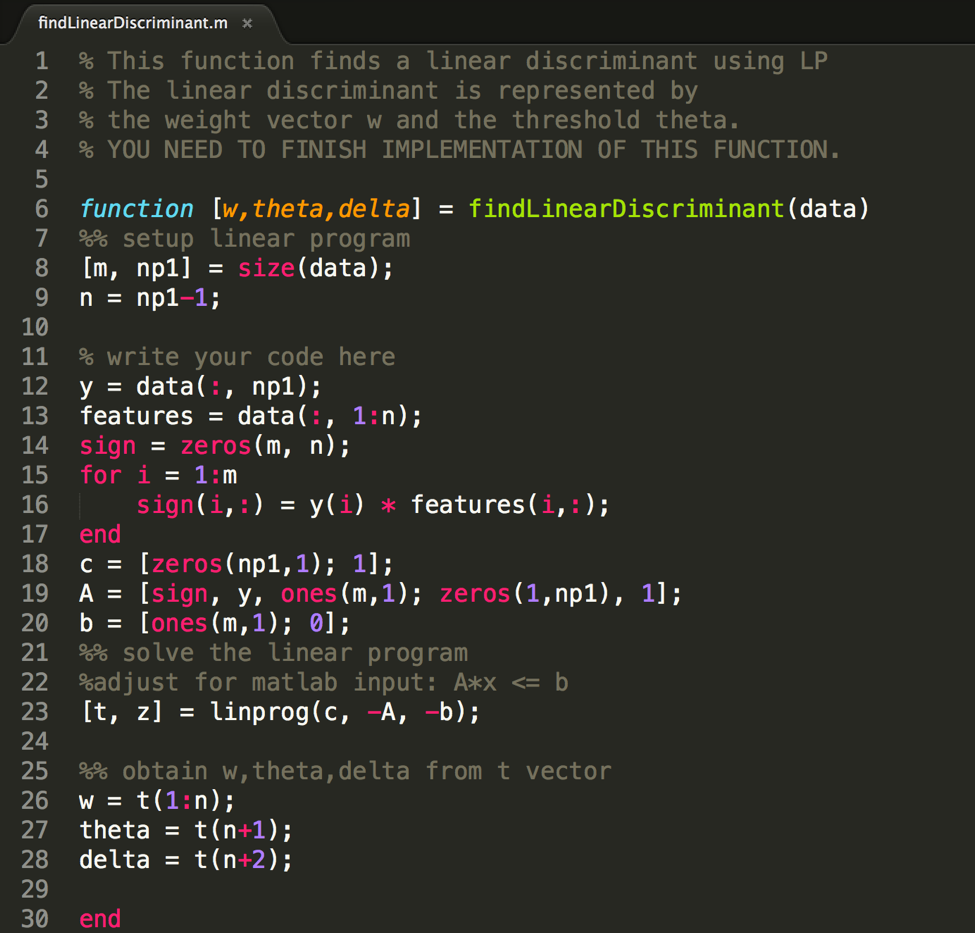
\includegraphics[width=13cm]{code_1} \\
			\item[b.2] \textbf{hw1sample2d.txt} \\
			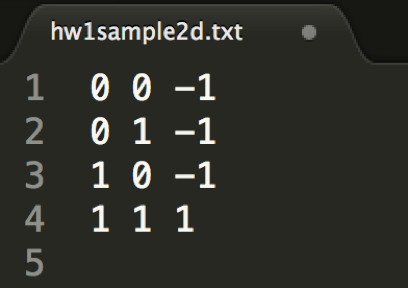
\includegraphics[width=5cm]{data_1.png}\\
			The dataset represents a monotone conjunction over two variables.\\\\
			\textbf{plot2dSeparator.m}\\
			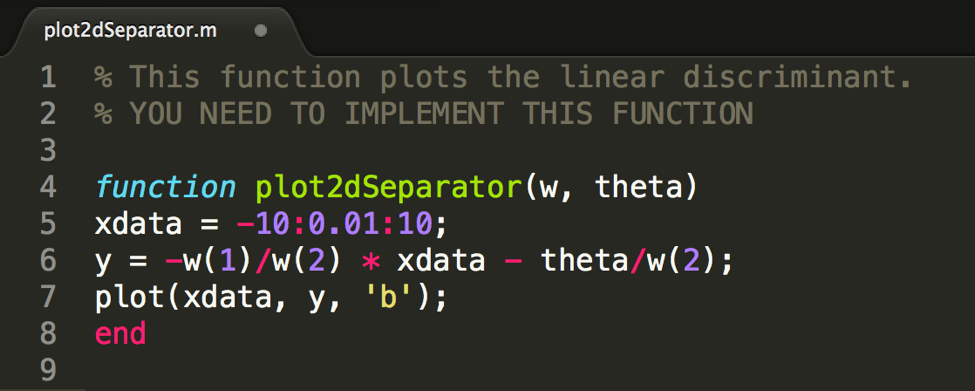
\includegraphics[width=13cm]{code_3}\\\\
			\textbf{two dimension separator:}\\
			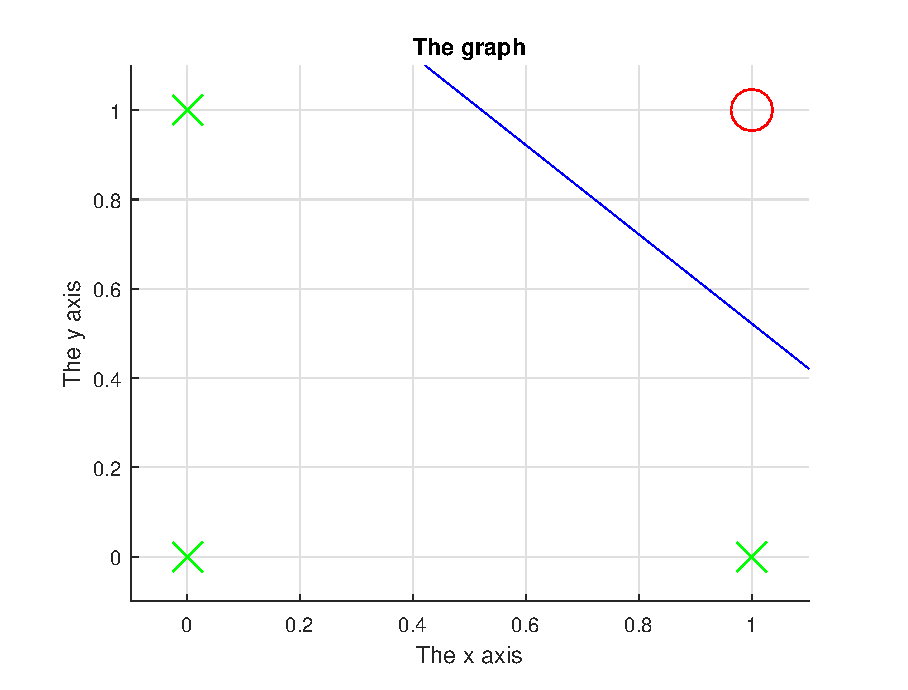
\includegraphics[width=13cm]{figure_1}\\
			$\theta=-90.2115$, $\delta = -1.5632e-13$\\
			$\vec{w} = [2.910,-2.050,0.178,190.520,0.140,-3.101,-2.953,-193.278,1.168,-8.894]$\\
			In this solution, $\delta \approx 0$ shows that the dataset is linearly separable. Since $x_4$ and $x_8$ are significantly larger than others, the label is mostly depent on $x_4$ and $\neg x_8$. The hyperplane should be $x_4 \land \neg x_8$. In this solution, $\theta << 0$ guarantees a negative ouput when $\vec{w} \vec{x}$ is small.\\
			\item[b.3] \textbf{computeLabel.m}\\
			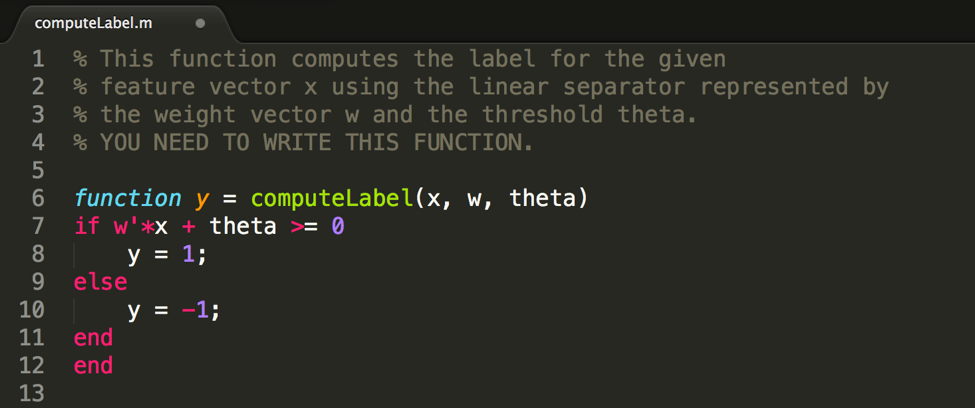
\includegraphics[width=13cm]{code_4}\\
			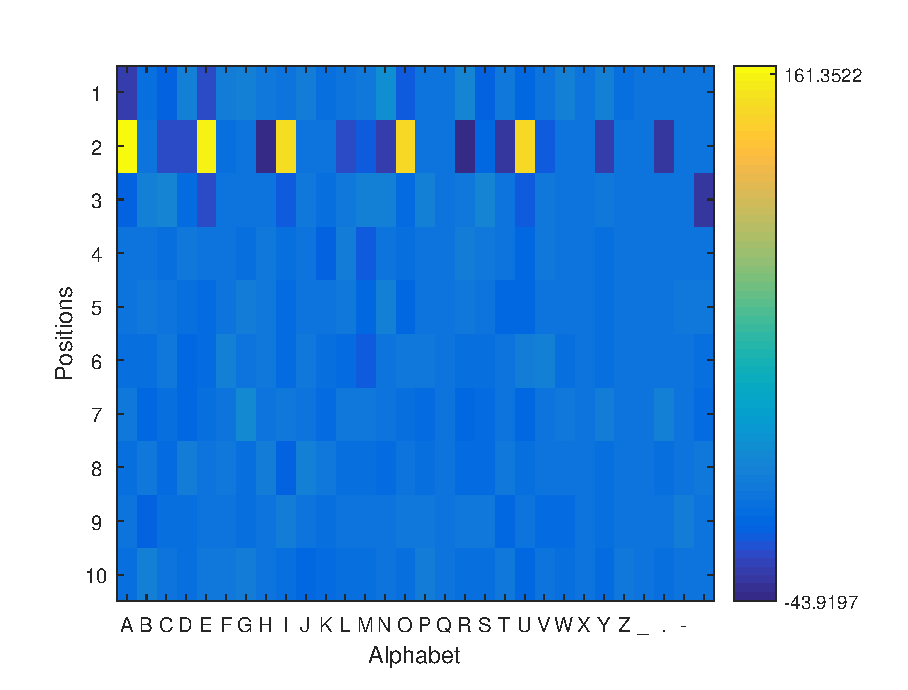
\includegraphics[width=10cm]{figure_3}\\
			($\delta=1.2619e-09$, $accuracyInTrain = 1$, $accuracyInTest = 1$)\\
			Since $\delta \approx 0$, there exists a hyperplane that separates dataset. This set of features shows a perfect accuracy in both training dataset and test dataset.\\\\
			\textbf{change the position from 1:10 to 3:10:}\\
			This change will ignore the first two positions, so the obvious yellow cube in image above will be ignored.\\
			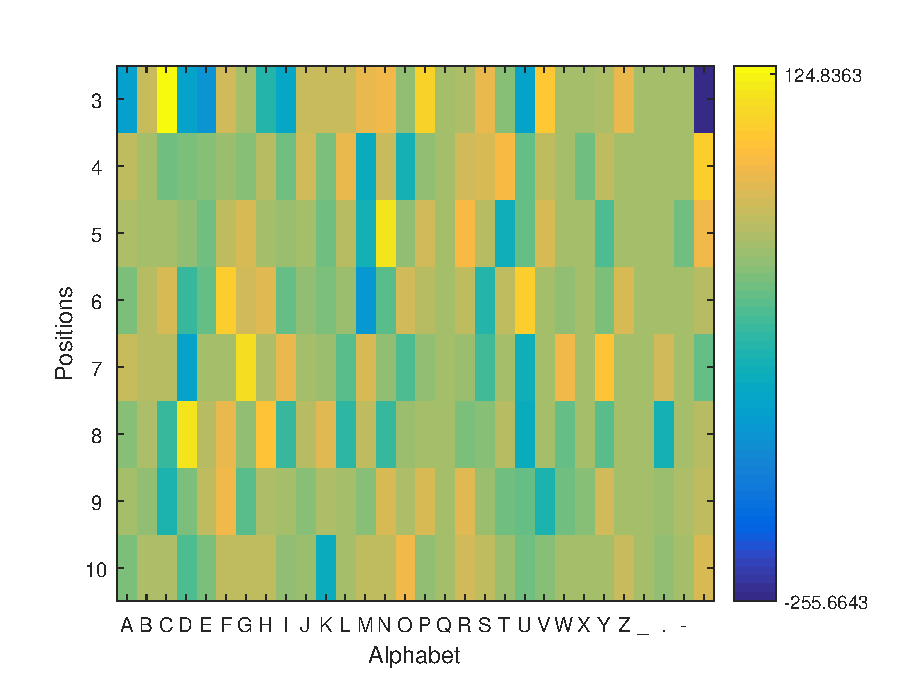
\includegraphics[width=10cm]{figure_4}\\
			($\delta=1.2179e-11$, $accuracyInTrain = 1$, $accuracyInTest = 0.7234$)\\
			Since $\delta \approx 0$, the new hyperplane separates the dataset. The accuracy for training dataset is $1$, but the accuracy for test is only $0.7$. There is no obvious feature under this alphabet and position.\\
			\item[b.4] \textbf{findLinearThreshold.m}\\
			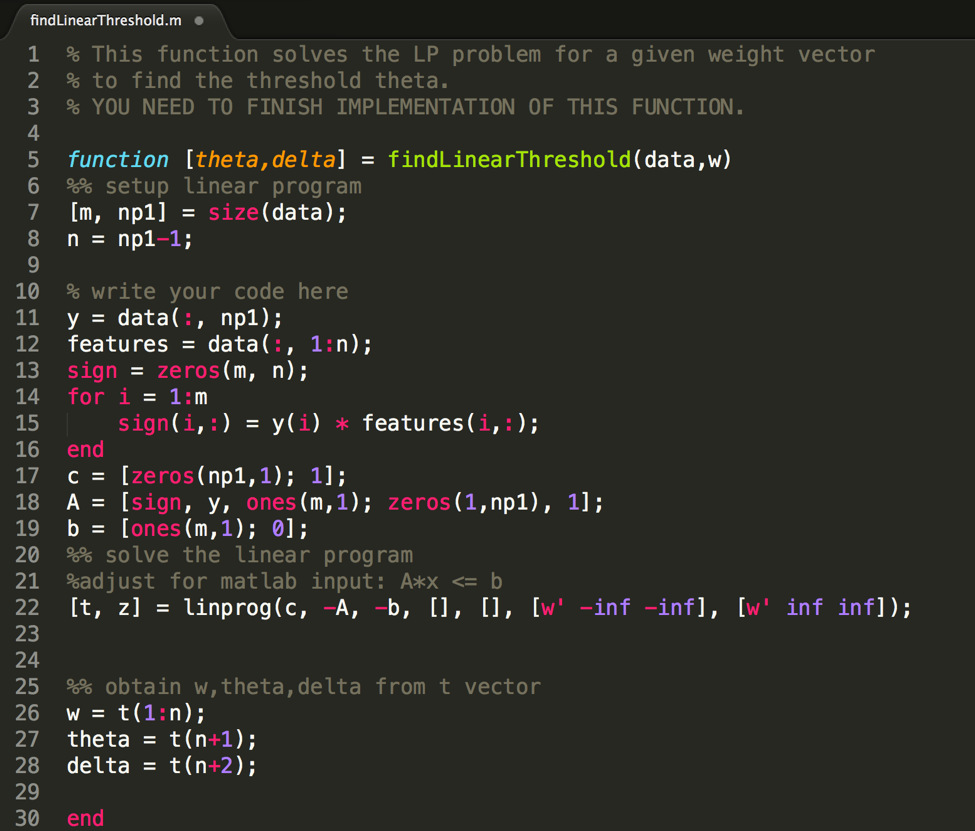
\includegraphics[width=13cm]{code_2}\\
			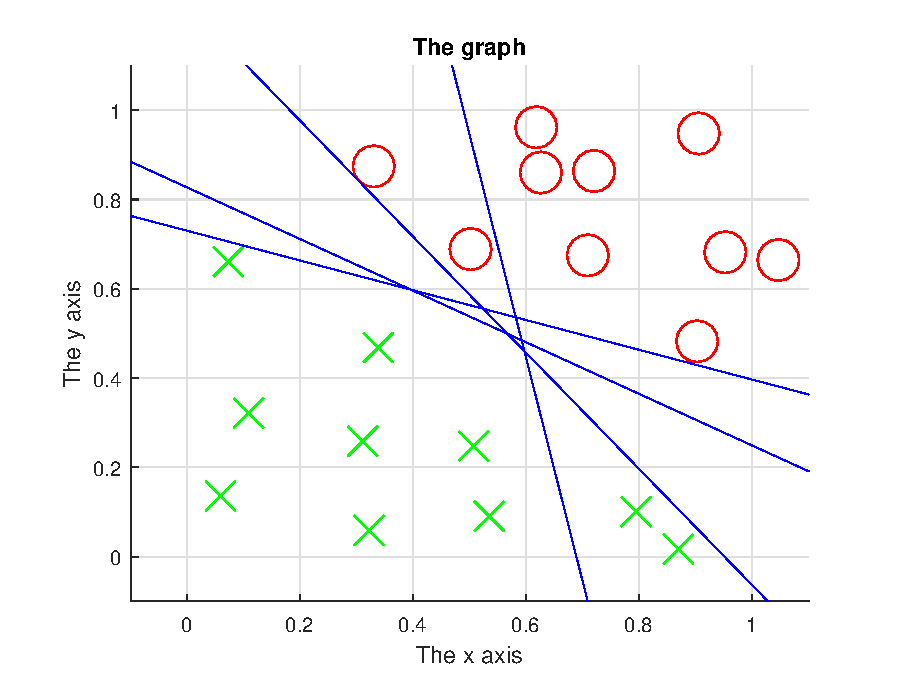
\includegraphics[width=13cm]{figure_2}\\
			($\delta_1=1.0658e-12$, $\delta_2=-2.2737e-13$, $\delta_3=-2.0009e-11$, $\delta_4=92.9650$)\\
			Among those four hypothesis, only three hypothesis sucessfully separates the dataset, ($\delta_4 >> 0$). The lines which left end located between $0.8$ and $1$ separates the dataset exactly. Since $\delta_4 >> 0$, the most vertical line fails to separates the dataset. Other two lines are closer to positive or negative examples. We can infer that there are multiply lines that can separate the dataset.
		\end{enumerate}
	\end{enumerate}
\end{enumerate}

\end{document}

